% Official template of the Research Group COMPUTATIONAL SOCIAL SCIENCE AND SYSTEMS ANALYTICS
% If you have problems after you did not find a solution on Stack Overflow or similar websites, or if you have an idea on how to improve this template,
% you can contact the author of the template: janina.lsd@uni-muenster.de

% ============================================================

% xxxxxxxxx  FIRST ADJUST THE FOLLOWING OPTIONS xxxxxxxxx
% a) the language of your thesis to either "english" or "german",
% b) the type of the thesis to either "bachelor", "master" or "seminar",
% c) and if the supervisor is equal to the principal supervisor
    % d1) It is possible that your thesis is supervised only by a member of the institute with a doctor title and no supervising professor. Then, you can use "postdoc" --> e.g., Dr. Lechtenbörger, ...
    % d2) else if there is a professor and a supervisor use "supervisor".
% d) If you are writing a thesis jointly with other students, set it to true for (seminar) paper with multiple authors.

\documentclass[
    language=german, % german english
    thesis=seminar, % seminar bachelor master
    supervisor=postdoc, % supervisor postdoc
    multiauthor=true, % true false 
    ]{settings/csssa-thesis}

% ============================================================
% Include all relevant information for the title page

\title{Interpreting Visual Attention: A Systematic Analysis of Eye-Tracking Data}
% If multiple authors write a (seminar) paper, use commas or newline (\\) to separate names, e-mail addresses, ids. Examples are given as comments below. 
\author{David Lika, }
%\author{Maja Mustermann, Max Musterfrau} \author{First Middle Last Name\\Second Student with somewhat longer Name}
\email{david.lika@uni-muenster.de, }
% Matriculation Number
\id{537160, }
% Information about the thesis and the course
\professor{Prof. Dr.-Ing. Grimme }
\supervisor{Prof. Dr.-Ing. Grimme }
% You only have to include the course if you are writing a seminar thesis
\course{Eyes Wide Scroll}
% Submission Date
\date{25.09.2025}

% Declare whether you used any AI-powered tools in your thesis. It will be added to the declaration of authorship which you have to sign. Default is given below, delete and add your text if you used any tools: 

\declarationTool{I hereby declare that I have not used any unauthorized assistance in the preparation of my thesis. In particular, I declare that I have not used any automatic writing aids such as \textit{Grammarly}, \textit{ChatGPT} or similar software tools to create, edit, or change essential parts of my thesis.}

% Examples for alternatives (If you used a tool for other purposes, add them below): 
% I hereby declare that I have used [Tool xyz] to check for spelling, grammar or plagiarism. .... 


% ============================================================


% ============================================================
% Place for adding additional packages (if required)
% 
% 
  
% ============================================================


% ============================================================
\begin{document}
\maketitlepage
\maketitle

% DON'T add a table of contents – that is not required for this thesis !!! Also, do not change the format of the template, just the content! 
\begin{quote}
    The eyes are not only passive receivers of visual stimuli, but active seekers of information guided by attention.
    {\textit{Alfed L. Yarbus (Eye Movemnet and Vision, 1967)}}
\end{quote}

\begin{abstract}
    \lipsum[1]
\end{abstract}

\section{Einführung}

Nachdem die Datenerhebung abgeschlossen war, erfolgte zunächst eine explorative Analyse des Materials.
In diesem ersten Schritt lag der Fokus darauf, einen umfassenden Überblick über die erhobenen Eye-Tracking-Daten zu gewinnen,
ohne bereits spezifische Annahmen oder Hypothesen zu verfolgen. 
Ziel war es, Strukturen, Auffälligkeiten und Muster sichtbar zu machen, die sich aus den Blickverläufen,
Fixationen und Sakkaden ergeben. Dazu wurden grundlegende Kennwerte betrachtet, wie etwa die mittlere Fixationsdauer,
die Verteilung der Blickpunkte über die Stimuli hinweg oder die zeitliche Dynamik des Blickverhaltens.
Diese explorative Phase diente insbesondere dazu, erste Einsichten in die Daten zu gewinnen,
mögliche Einflussfaktoren zu identifizieren und relevante Variablen für eine weiterführende Analyse einzugrenzen.
Gleichzeitig konnten wir dadurch prüfen, ob die Datenqualität den Anforderungen entspricht und ob sich erwartungsgemäß
interpretierbare Strukturen abzeichnen. 

Aufbauend auf diesen ersten Befunden folgte eine systematische Analyse.
Während die explorative Untersuchung noch eher offen und hypothesengenerierend angelegt war,
stand in diesem zweiten Schritt die gezielte Überprüfung einer klar formulierten Fragestellung im Vordergrund.
Auf Basis der im explorativen Teil gewonnenen Einsichten formulierten wir eine spezifische Hypothese,
die sich auf ein bestimmtes Muster im Blickverhalten bezog. Diese Hypothese wurde anschließend mit geeigneten
statistischen Verfahren überprüft. Dadurch konnten wir nicht nur unsere anfänglichen Beobachtungen absichern,
sondern auch präzise Aussagen darüber treffen, ob die vermuteten Zusammenhänge tatsächlich empirisch gestützt werden können. 

Durch das zweistufige Vorgehen - zunächst explorativ, dann hypothesengeleitet - wurde sichergestellt,
dass wir sowohl unvoreingenommene Einblicke in das Datenmaterial erhielten als auch die Möglichkeit hatten,
spezifische Annahmen fundiert zu prüfen. Dieses Vorgehen verbindet Offenheit gegenüber unerwarteten Mustern
mit wissenschaftlicher Stringenz bei der Hypothesenprüfung und ermöglicht damit eine differenzierte
Interpretation der Eye-Tracking-Daten

\section{Clustern}
\textbf{Hypothese:} Fixationsmuster lassen sich in klar unterscheidbare Cluster einteilen, die mit den Bildmerkmalen korrespondieren. 

\section{Betrachtungsdauer}
\subsection{Zeitpunkt}
 \textbf{Hypothese:} Die Betrachtungsdauer von später gezeigten Bildern ist geringer als Bilder, die früh gezeigt werden. 

Um diese Hypothese zu testen, wurde ein lineares Mixed-Effects-Modell verwendet, 
welches die Reihenfolge des Zeigens (als erstes gezeigt = 1, als zweites = 2 usw.) 
als Prädiktor nimmt und einen normalverteilten, zufälligen Interzept hinzuzieht,
welcher unterschiedliche Grundniveaus (manche Personen schauen generell länger auf Bilder als andere) berücksichtigt.
Für eine stabilere Schätzung wurden die Betrachtungsdauern log-transformiert. Die Berechnung wurde mit Python durchgeführt, 
mithilfe des „mixedlm“-Modells der „statsmodels.formula.api“-Bibliothek. Die Daten wurden durch numpy.log1p() log-transformiert.

Bei diesem linearen Mixed-Effects-Modell ist eine Steigung der Reihenfolge von 
$\beta \approx -0.00071$ mit einem 95\%-Konfidenzintervall 
$[-0.000837;\,-0.000579]$ ermittelt worden, was einem Abfall der Betrachtungsdauer 
von ungefähr $0.071\%$ pro Bild und auf $152$ Bilder gesehen ca. $10.792\%$ entspricht. 
Das bedeutet, dass jedes Bild (in Sekunden umgerechnet) um ca.\ $0.0075$ Sekunden pro Schritt 
kürzer betrachtet wird als das vorherige. Auf $152$ Bilder gesehen ergibt das 
einen gesamten Abfall von ca.\ $1.14$ Sekunden vom ersten auf das letzte Bild. 
Weitere Daten dieses Modells sind wie folgt:

\begin{itemize}
  \item $SE = 0.0000658$
  \item $t = \beta / SE = -10.75$
  \item Zweiseitig $p = 5.6 \cdot 10^{-27}$
  \item Einseitig für „später = kürzer“ $p = 2.8 \cdot 10^{-27}$
\end{itemize}


Die sehr kleine Standardabweichung (SE) zeugt von einer sehr präzisen Schätzung der Steigung.  
Außerdem ist der t-Wert extrem (negativ) groß und die p-Werte beide extrem nahe an null,
was auf einen hochsignifikanten negativen Trend schließen lässt. Somit bestätigen unsere
Daten die oben genannte Hypothese. In Abbildung \ref{fig:lineareAppox} ist eine lineare Approximation der
Betrachtungsdauer zu sehen. Sie veranschaulicht die Bestätigung unserer Hypothese. 

\begin{figure}[h]
    \centering
    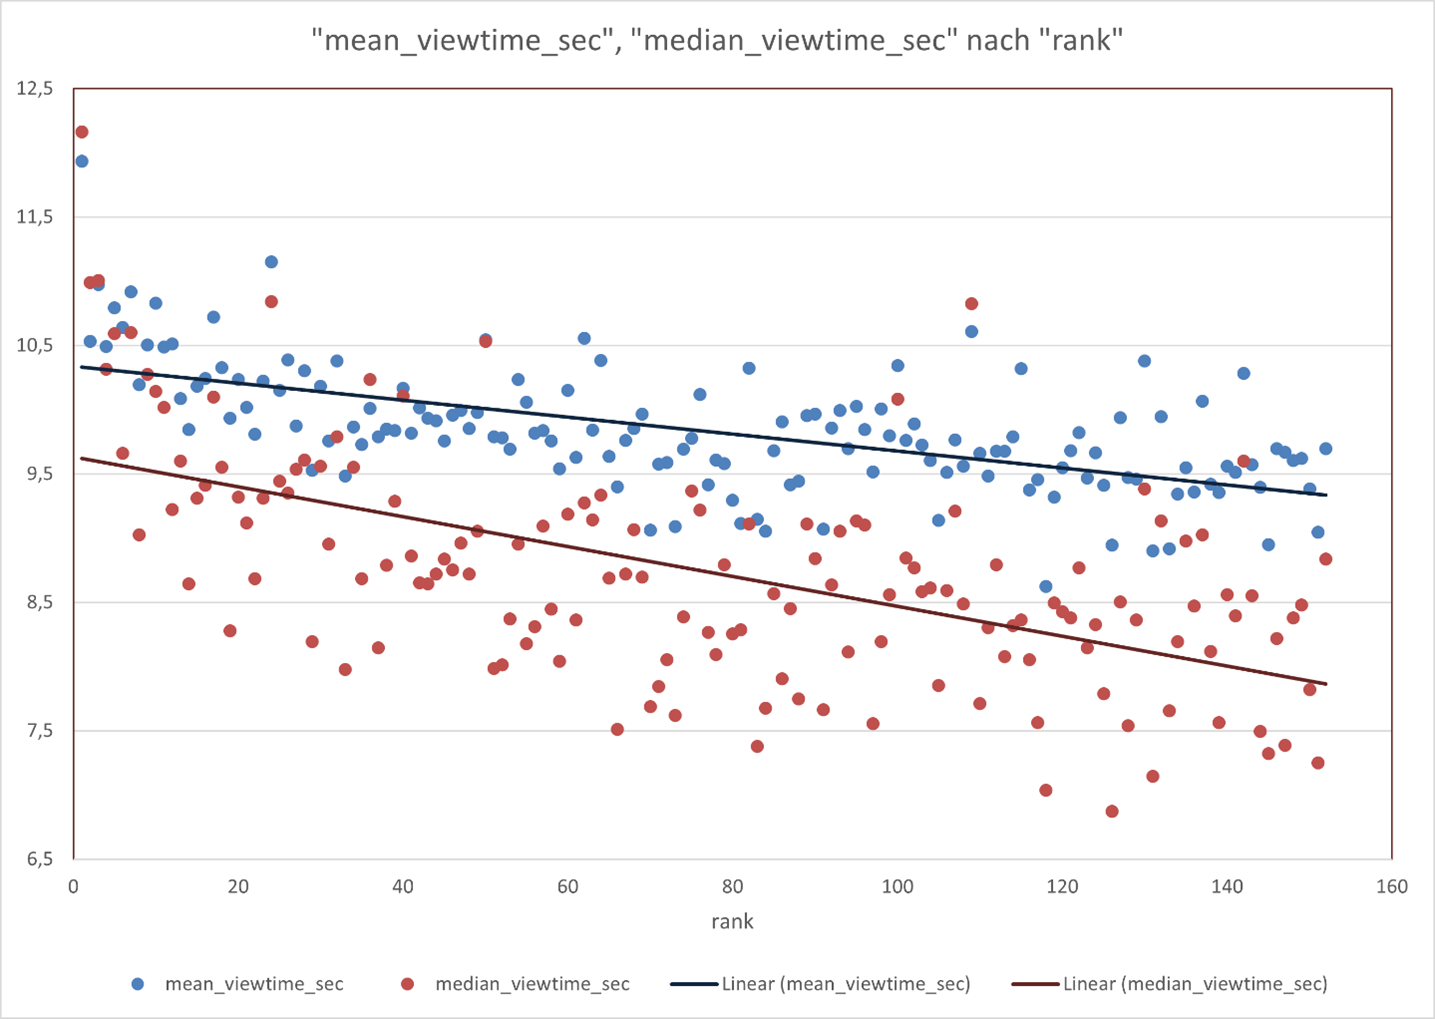
\includegraphics[width=\linewidth,height=0.8\textheight,keepaspectratio]{figures/Bild1.png}
    \caption{Lineare Approximation der Betrachtungsdauer in Abhängigkeit vom Zeitpunkt der Bildpräsentation. Durchschnitt (blau) und Median (rot) sind dargestellt.}
    \label{fig:lineareAppox}
\end{figure}

Diese Hypothese ist uns bereits vor der Durchführung unserer Studie in den Sinn gekommen, 
weshalb wir vorab bereits allen Probanden eine zufällige Reihenfolge der Bilder gezeigt haben, 
um bei Bestätigung dieser Hypothese keine Ergebnisse erhalten, die mit einem Bias versehen sind. 
Durch die zufällige Reihenfolge ist davon auszugehen, dass jedes Bild gleichhäufig an den entsprechenden 
Zeitpunkten gezeigt wurde, weshalb jedes Bild denselben Bias haben sollte und dieser sich somit ausgleicht. 
Zukünftige Studien sollten dies ebenfalls beachten. 

\subsection{Kategorien}
\textbf{Hypothese:} Die Kategorien eines Bildes haben Einfluss auf die Betrachtungsdauer im Median 

Um diese Hypothese zu testen, verglichen wir zunächst die Mediane über unsere Kategorien hinweg. 
Zwischen unseren Kategorien (Personen, Politik, Memes, Orte und Text) sowie ihren Kombinationen 
fallen bereits einige Kategorien als besonders prominent auf. Generell ist auffällig, dass 
Kombinationen mit Text längere Betrachtungsdauer aufweisen als der Konterpart ohne Text (Abb. \ref{fig:katDauer}) 

\begin{figure*}[ht]
    \centering
    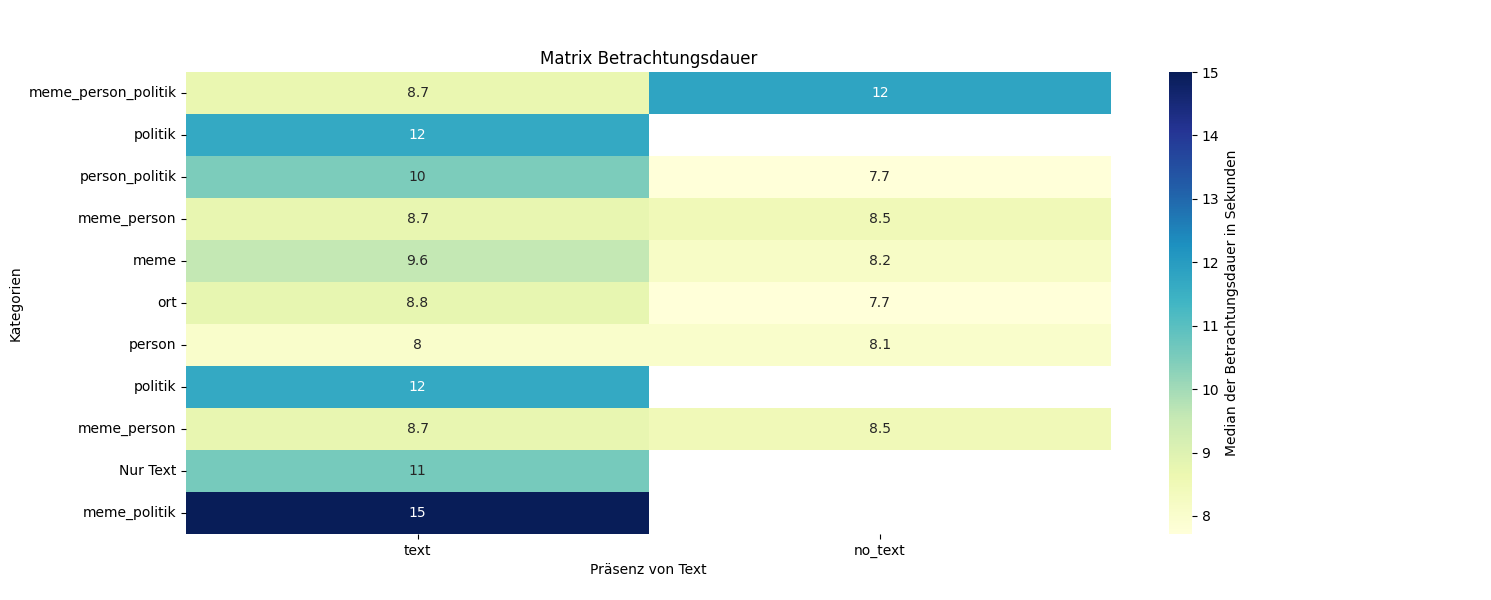
\includegraphics[width=0.8\textwidth,height=0.8\textheight,keepaspectratio]{figures/Bild2.png}
    \caption{Die Kategorien mit der jeweiligen durchschnittlichen Betrachtungsdauern}\label{fig:katDauer}
\end{figure*}

Diese Tatsache hing nach näherer Betrachtung allerdings im Wesentlichen von der Menge an Text ab,
den die Probanden in der Regel sorgfältig lasen. Abb. \ref{fig:katMatrix} zeigt die Betrachtungsdauer der einzelnen 
Kategorien aufgeschlüsselt auf Text und keinen Text. 

\begin{figure}[h]
    \centering
    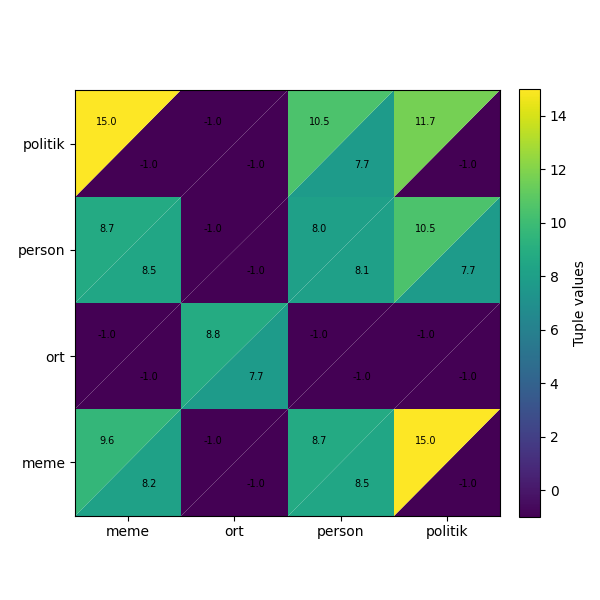
\includegraphics[width=0.8\linewidth,height=0.8\textheight,keepaspectratio]{figures/Bild3.png}
    \caption{Jedes Feld zeigt die Kombination zweier Kategorien, mit dem Wert für "Text" linksoben und "Ohne Text" rechtsunten}\label{fig:katMatrix}
\end{figure}

Daher versuchten wir, den Einfluss der Textlänge herauszufiltern. Als erste Lösung bereinigten 
wir die Betrachtungsdauer um die Anzahl der Wörter mit folgender Formel:

\[
\text{Dauer}_{\text{bereinigt}} = \frac{\text{Dauer}_{\text{gemessen}} - 5}{\text{Wörteranzahl}}
\]


Die resultierenden relativen Betrachtungsdauern sind in Abbidlung \ref{fig:bild27} dargestellt, 
wobei ein Vergleich mit Bildern ohne Text wegen fehlender Vergleichbarkeit außen vor gelassen wurde.

\begin{figure}[h]
    \centering
    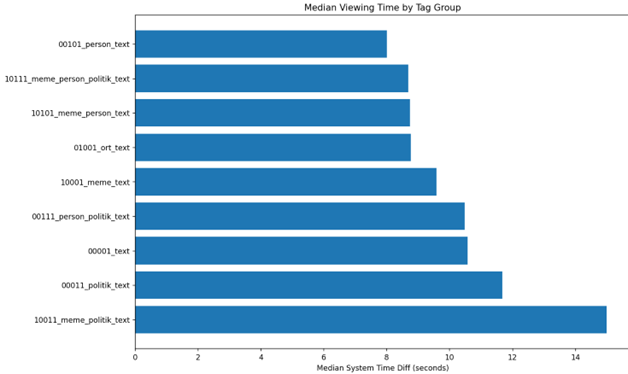
\includegraphics[width=\linewidth,height=0.8\textheight,keepaspectratio]{figures/Bild31.png}
    \caption{Median der Betrachtungsdauer pro Gruppe}
    \label{fig:bild27}
\end{figure}

Eine Möglichkeit, um den Einfluss jeder Kategorie auf die Betrachtungsdauer zu ermitteln, 
ist die Regression. In unserem Fall lag eine Zensierung der Daten, also eine Beschränkung 
auf ein bestimmtes Intervall von 5 bis 15 Sekunden vor, weshalb eine gewöhnliche Regression 
ungeeignet schien. Eine Alternative stellte die Überlebenszeitanalyse und insbesondere das Modell 
für beschleunigte Ausfallzeiten (AFT) dar, das mit zensierten Werten umgehen kann.

Wir verglichen die AICs verschiedener AFT-Modelle und wählten den LogNormal-AFT-Fitter, 
der den besten AIC besaß. Die Ergebnisse zeigt Tabelle 1. Es stellte sich heraus, dass die Anzahl 
der Wörter mit einer Sekunde je weiterem Wort und die Kategorie Politik mit zusätzlichen 1,07 Sekunden 
bei Auftreten signifikant auf die Betrachtungsdauer einwirken.

\begin{table}[htbp]
\centering
\begin{tabular}{lcc}
\hline
\textbf{Kategorie} & \textbf{Koeffizient} & \textbf{p-Wert} \\
\hline
Ort          & 1.02 & 0.32      \\
Person       & 1.05 & 0.01      \\
Meme         & 1.03 & 0.12      \\
Politik      & 1.07 & $<0.005$ \\
Wörteranzahl & 1.01 & $<0.005$ \\
\hline
\end{tabular}
\caption{Regressionsergebnisse: Koeffizienten und Signifikanzniveaus für verschiedene Kategorien.}
\label{tab:kategorien}
\end{table}

\section{Bildmerkmale}
\subsection{Kontraste}

\textbf{Hypothese:} Hoher Bildkontrast ist positiv mit der Fixationsanzahl und -dauer korreliert. 

\subsubsection{Ansatz \& Ergebnisse}
Wir untersuchen, ob und wie Bildkontrast mit Blickverhalten zusammenhängt: 
\begin{itemize}
    \item Werden kontrastreichere Bilder öfter fixiert? 
    \item Dauern Fixationen länger oder kürzer? 
\end{itemize}
Dazu kombinieren wir zwei Komplementär-Metriken auf dem Bild mit zusammengefassten Fixationsdaten. 

Fixationen werden wie folgt berechnet \cite{Salvucci_IdentifyingFixations}. 

\subsubsection{Bildmetriken}
\paragraph{RMS-Kontrast.} 
Misst die globale Helligkeitsspanne eines Bildes. Mathematisch: die Standardabweichung der auf $[0,1]$ 
normalisierten Grauwerte. Hoher RMS $\rightarrow$ große Unterschiede zwischen hell und dunkel, unabhängig von deren Position im Bild. 

\paragraph{Laplace (normalisierte Varianz).}
Misst Kanten/Feinstruktur/Schärfe. Pipeline: 
\begin{enumerate}[label=(\alph*)]
    \item optionale Gauß-Glättung ($\sigma$) zur Rauschreduktion, 
    \item Laplace-Filterung, 
    \item Berechnung der Varianz des Laplace-Bildes, geteilt durch die Varianz des (geglätteten) Intensitätsbildes. 
\end{enumerate}
Hoher Wert $\rightarrow$ viele/kräftige Kanten und feine Details. 
RMS und Laplace fassen damit unterschiedliche Aspekte von „Kontrast“: Gesamtlautstärke vs. Detailreichtum.  

\vspace{0.3em}
\noindent
\textit{Wissenschaftliche Grundlage:} \cite{Kukkonen1993}. 

\subsubsection{Fixationsmetriken}
Pro Bild aggregieren wir die Fixationsdaten über Personen mit einem getrimmten Mittel (5–95\,\%): 
\begin{itemize}
    \item $n\_fix\_mean\_trim$: mittlere Anzahl Fixationen, 
    \item $tot\_dur\_mean\_trim$: mittlere Gesamtdauer aller Fixationen (ms), 
    \item $med\_dur\_mean\_trim$: mittlerer Median der Fixationsdauer (ms) – robust gegen Ausreißer. 
\end{itemize}

\subsubsection{Korrelationen}
Wir korrelieren pro Bild die Kontrastwerte mit den drei Blick-Kennzahlen (Pearson; $n \approx 152$ Bilder). Die wichtigsten Zusammenhänge:
siehe Abbildung \ref{fig:bild4} bis \ref{fig:bild9}

\begin{figure}[h]
    \centering
    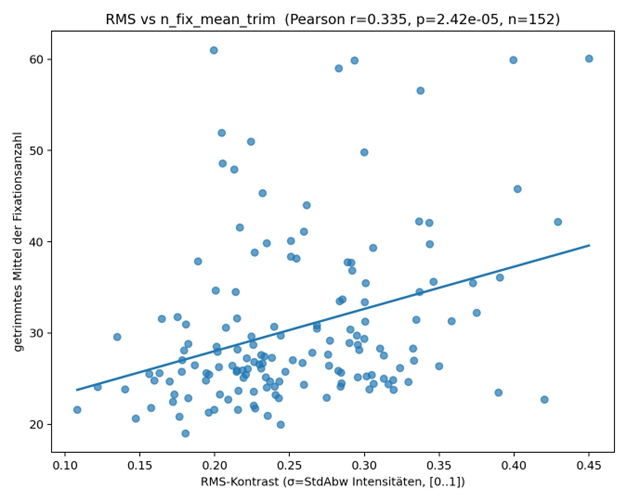
\includegraphics[width=\linewidth,height=0.8\textheight,keepaspectratio]{figures/Bild4.png}
    \caption{RMS $\rightarrow n\_fix\_mean\_trim$: $r \approx 0.34$, $p \ll .01$ \\
          Höherer globaler Kontrast geht mit mehr Fixationen einher. }\label{fig:bild4}
\end{figure}

\begin{figure}[h]
    \centering
    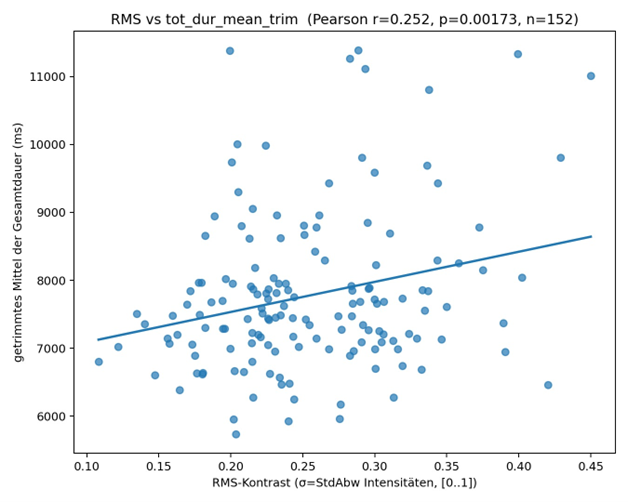
\includegraphics[width=\linewidth,height=0.8\textheight,keepaspectratio]{figures/Bild5.png}
    \caption{ RMS $\rightarrow tot\_dur\_mean\_trim$: $r \approx 0.25$, $p \ll .01$ \\
          Leicht längere Gesamtdauer bei höherem RMS. }\label{fig:bild5}
\end{figure}
\begin{figure}[h]
    \centering
    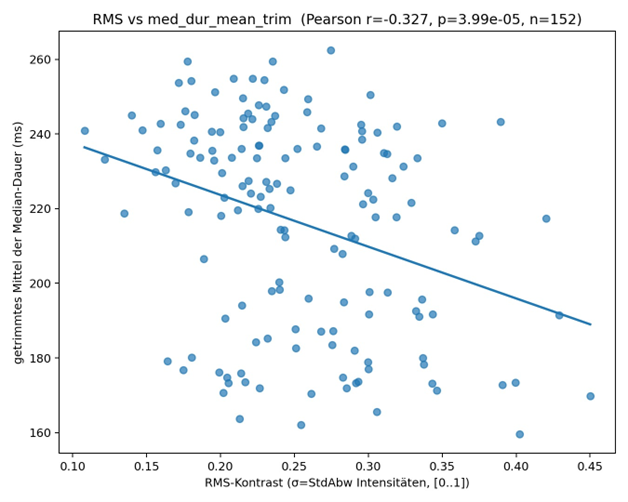
\includegraphics[width=\linewidth,height=0.8\textheight,keepaspectratio]{figures/Bild6.png}
    \caption{ RMS $\rightarrow med\_dur\_mean\_trim$: $r \approx -0.33$, $p \ll .01$ \\
          Kürzere typische (Median-)Fixationen bei mehr Kontrast. }\label{fig:bild6}
\end{figure}
\begin{figure}[h]
    \centering
    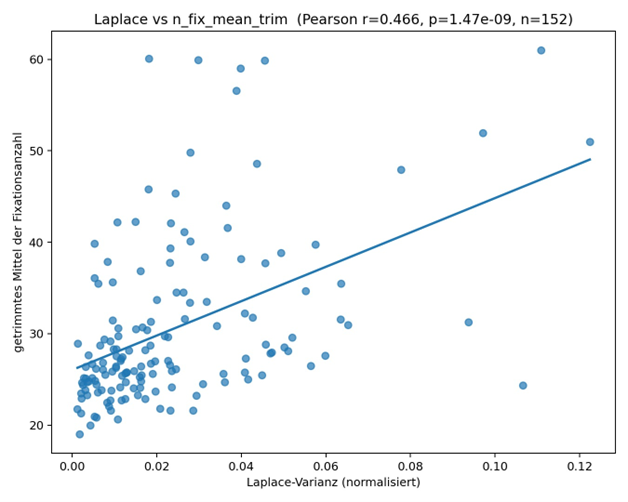
\includegraphics[width=\linewidth,height=0.8\textheight,keepaspectratio]{figures/Bild7.png}
    \caption{Laplace $\rightarrow n\_fix\_mean\_trim$: $r \approx 0.47$, $p \ll .001$ \\
          Stärkster positiver Zusammenhang: detail-/kantenreiche Bilder werden deutlich häufiger fixiert. }\label{fig:bild7}
\end{figure}
\begin{figure}[h]
    \centering
    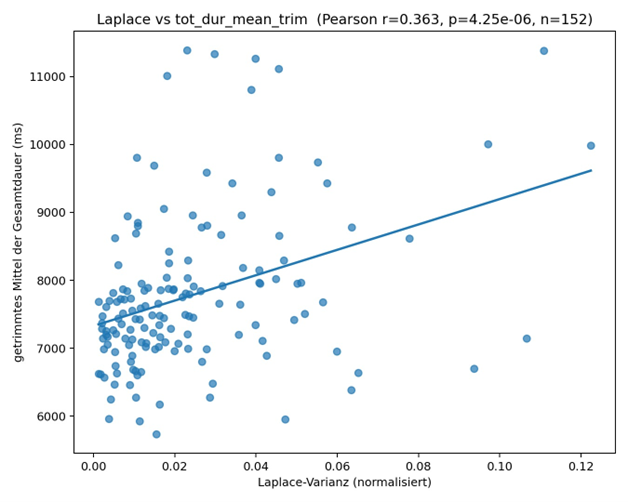
\includegraphics[width=\linewidth,height=0.8\textheight,keepaspectratio]{figures/Bild8.png}
    \caption{Laplace $\rightarrow tot\_dur\_mean\_trim$: $r \approx 0.36$, $p \ll .001$ \\
          Mehr Gesamtdauer mit steigender Kantenstärke.  }\label{fig:bild8}
\end{figure}
\begin{figure}[h]
    \centering
    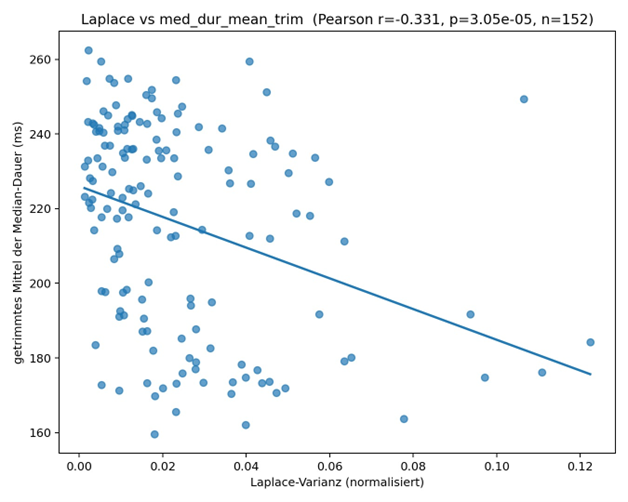
\includegraphics[width=\linewidth,height=0.8\textheight,keepaspectratio]{figures/Bild9.png}
    \caption{Laplace $\rightarrow med\_dur\_mean\_trim$: $r \approx -0.33$, $p \ll .01$ \\
          Kürzere Einzel-Fixationen bei mehr Details.  }\label{fig:bild9}
\end{figure}

\subsubsection{Interpretation}
Bilder mit hohem RMS oder hohem Laplace-Wert ziehen den Blick häufiger an (mehr Fixationen) und führen trotz kürzerer Einzel-Fixationen zu mehr Gesamtdauer – konsistent mit einem \textit{Scanning-/Exploration-Muster}: Viele visuelle Ankerpunkte (Kanten, Texturen, Beschriftungen) werden nacheinander kurz begutachtet. 

Dass Laplace stärker mit der Fixationsanzahl korreliert als RMS, deutet darauf hin, dass Kanten/Feinstruktur (und nicht nur globale Helligkeitsspannen) ein besonders wirksamer Treiber für Aufmerksamkeit sind. Dies deckt sich mit der Literatur \cite{SaliencyPrediction_JoV}.

\subsubsection{Limitationen \& nächste Schritte}
Korrelation $\neq$ Kausalität; Kategorien (z.\,B. Text) könnten Kontrast und Blickverhalten gemeinsam beeinflussen. Sinnvoll sind: 
\begin{enumerate}[label=(\alph*)]
    \item Analysen innerhalb von Kategorien, 
    \item multiple Regressionen mit RMS + Laplace + Kategorie-Dummies, 
    \item Spearman als Rangkorrelation für Robustheit, 
    \item Sensitivitätsanalysen für den Glättungs-$\sigma$ beim Laplace-Maß. 
\end{enumerate}

\subsubsection{Take-away}
\begin{itemize}
    \item RMS liefert ein stabiles Maß für globalen Kontrast. 
    \item Laplace quantifiziert Details/Kanten. 
\end{itemize}
Gemeinsam erklären sie plausibel, warum bestimmte Bilder häufiger und länger betrachtet werden, obwohl einzelne Fixationen kürzer ausfallen. 

Ein nächster Schritt wäre die Umsetzung einer linearen Regression, um anhand von RMS- und Laplace-Werten die Fixationskennzahlen vorherzusagen. 

\section{Wiederholte Betrachtung von Bildelementen}

\textbf{Hypothese:} Bildkategorien haben Einfluss auf die Rekurrenz der Fixationen 

\subsection{Methodik}
Recurrence quantification analysis (RQA) nach \citeauthor{Anderson2013-oj}. 
Kurzfassung: Zu jeder Bildbetrachtung wird aus der zugehörigen Fixationssequenz 
eine Rekurrenz Matrix berechnet. Aus dieser wiederum lassen sich die Metriken recurrence, 
determinism, laminarity (jeweils in Prozent) und center of recurrence mass (corm) bestimmen. 
Diese wurden zu allen erhobenen Eye-Tracker Daten berechnet, auf Korrelation überprüft 
und zu Histogrammen (nach unterschiedlichen Bildkategorien) aggregiert.

\subsection{Ergebnisse und mögliche Interpretation}
Abbildung \ref{fig:Bild10a} und \ref{fig:Bild10b} dienen als Beispiel dafür, wie sich die Metriken ergeben. 
Abbildung \ref{fig:Bild11} zeigt die Verteilung der Metriken als Histogramm. Auffällig ist 
die hohe Anzahl an „Null-Werten“ bei determinism und laminarity. 
In der Korrelationsmatrix in Abbildung \ref{fig:Bild12} lässt sich erkennen, dass diese zum 
Teil mit einer niedrigen recurrence korrelieren (mehr dazu im Vergleich zwischen Bildkategorien nach Ort). 
Denn: Je weniger sich Fixationen wiederholen, desto seltener wiederholen sich 
Fixationssequenzen (determinism) und desto seltener werden AOIs im Detail gescannt (laminarity). 

\begin{figure}[ht]
    \centering
    \begin{subfigure}{0.49\textwidth}
        \centering
        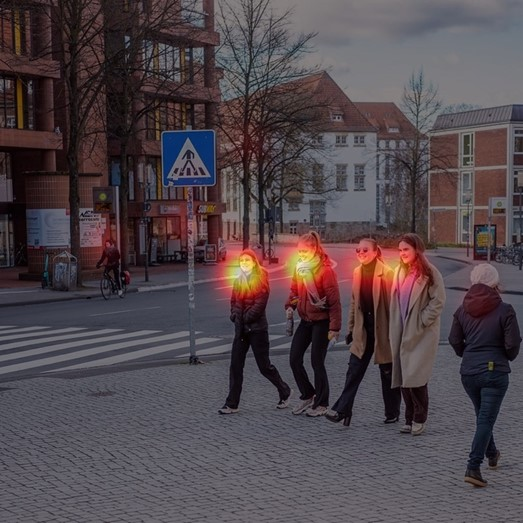
\includegraphics[width=0.8\textwidth]{figures/Bild10.jpg}
        \caption{Proband 35 mit Bild 37 und Heatmap}\label{fig:Bild10a}
    \end{subfigure}
    \begin{subfigure}{0.49\textwidth}
        \centering
        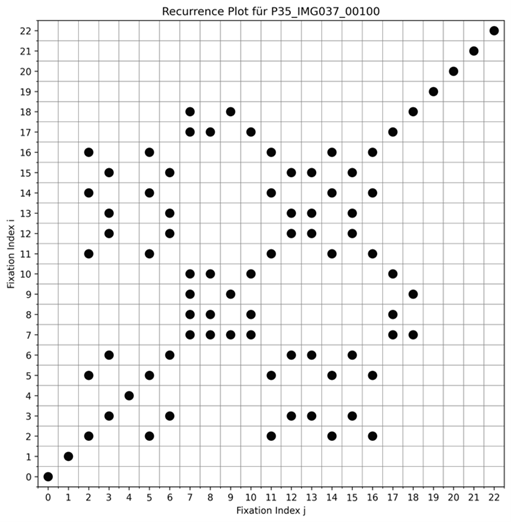
\includegraphics[width=0.8\textwidth]{figures/Bild11.png}
        \caption{Rekurrenz Plot zu Abbildung \ref{fig:Bild10a}}\label{fig:Bild10b}
    \end{subfigure}\label{fig:Bild10}
    \caption{N = 23, R = 29, REC = 11.46\%, DET = 62.07\%, LAM = 25.86\%, CORM = 29.78\%}
\end{figure}

\begin{figure*}[ht]
    \centering
    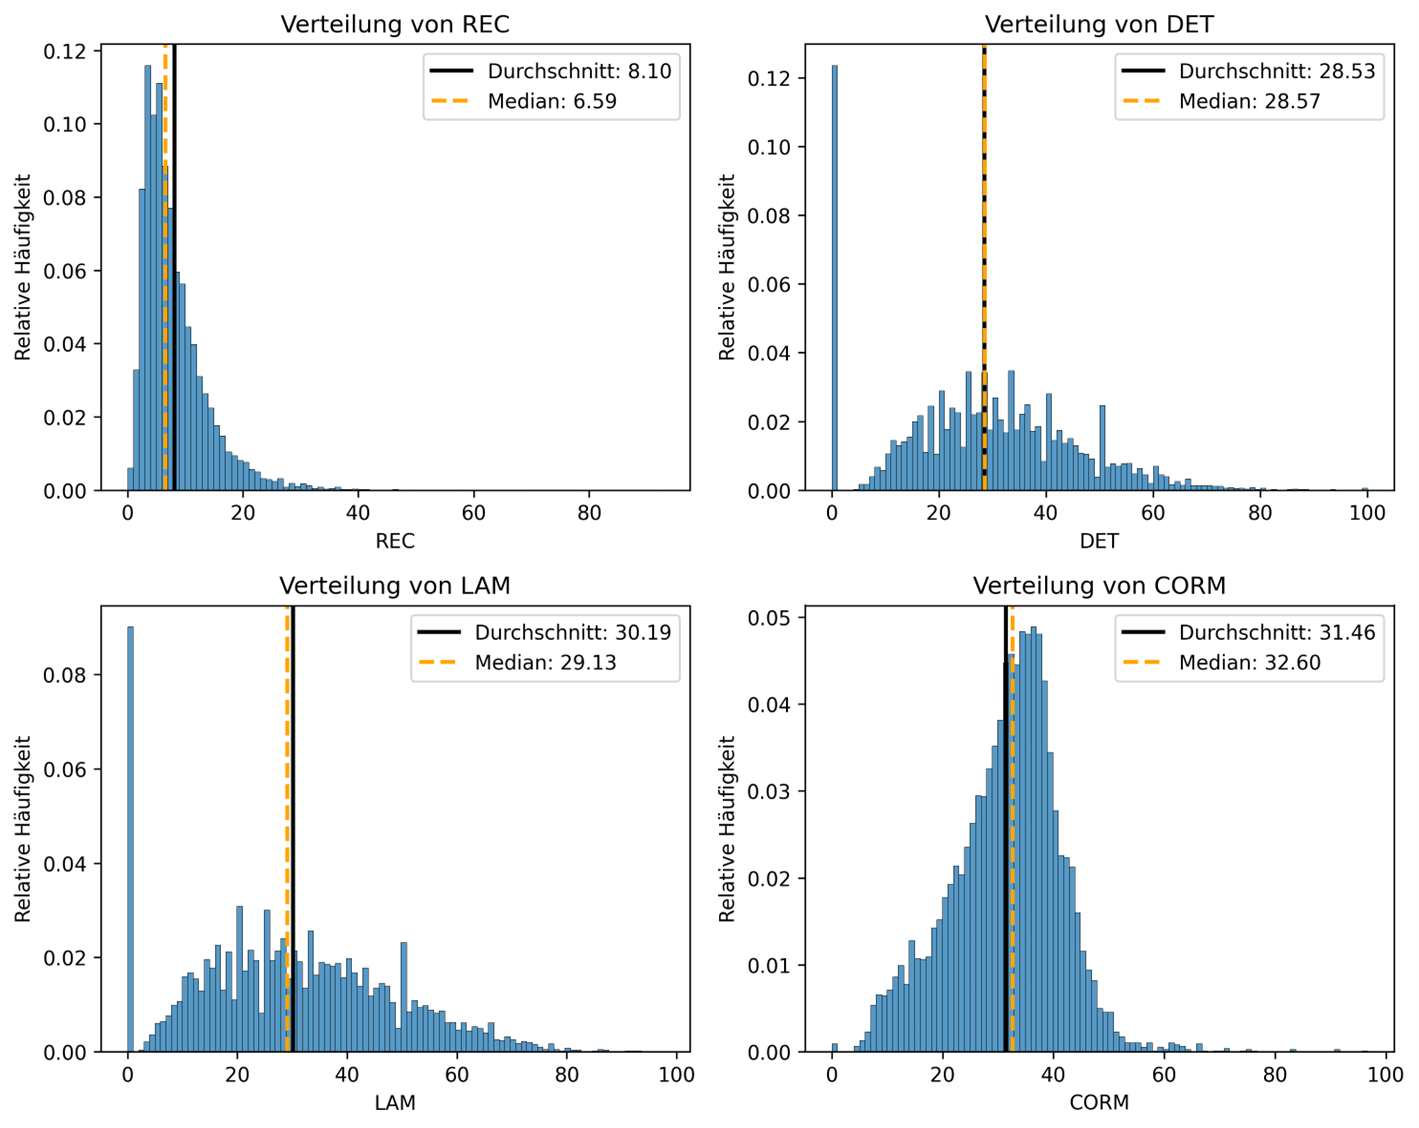
\includegraphics[width=0.8\textwidth,height=0.8\textheight,keepaspectratio]{figures/Bild12.png}
    \caption{Histogramme der Metriken aller Daten}\label{fig:Bild11}
\end{figure*}

\begin{figure*}[ht]
    \centering
    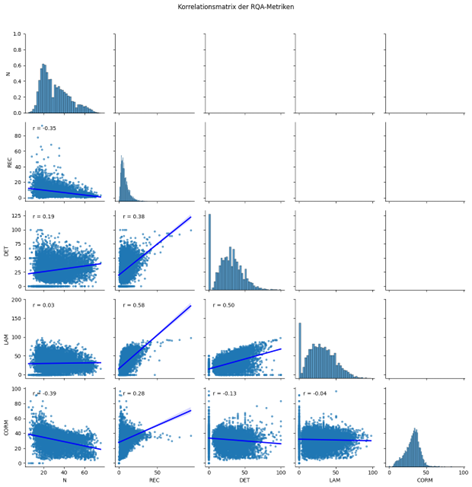
\includegraphics[width=0.8\textwidth,height=0.8\textheight,keepaspectratio]{figures/Bild13.png}
    \caption{Korrelationsmatrix der Metriken + Histogramm}\label{fig:Bild12}
\end{figure*}

Hohe determinism Werte können sich andererseits bspw. 
aus dem wiederholten Lesen von Text ergeben (Abb. \ref{fig:Bild13a} und ref{fig:Bild13b}). 
Zusätzlich können hohe Ausreißer entstehen, wenn sich der Proband nur eine AOI anschaut (Abb. \ref{fig:Bild14a} und \ref{fig:Bild14b}). 

\begin{figure}[ht]
    \centering
    \begin{subfigure}{0.49\textwidth}
        \centering
        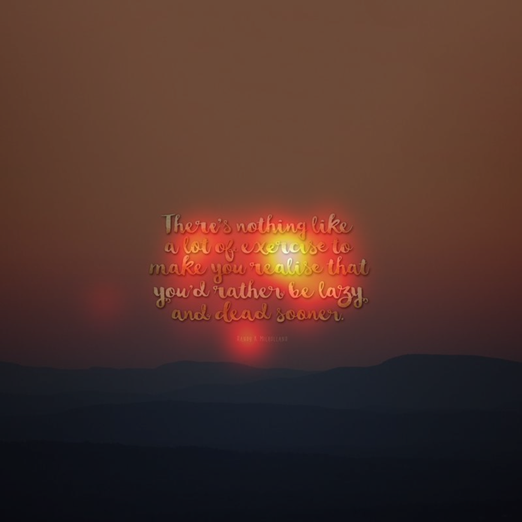
\includegraphics[width=0.8\textwidth]{figures/Bild14.png}
        \caption{Proband 42 mit Bild 128 und Heatmap}\label{fig:Bild13a}
    \end{subfigure}
    \begin{subfigure}{0.49\textwidth}
        \centering
        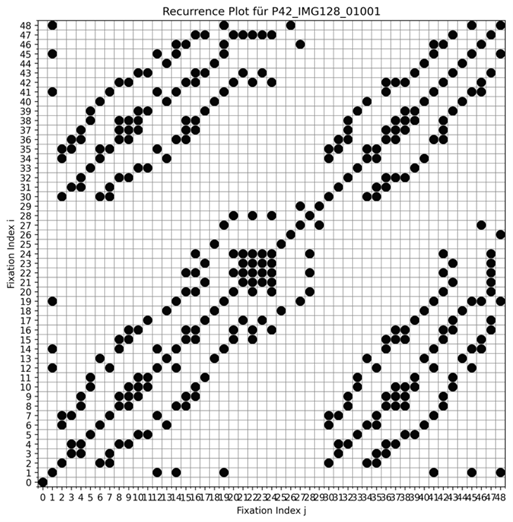
\includegraphics[width=0.8\textwidth]{figures/Bild15.png}
        \caption{Rekurrenz Plot zu Abbildung \ref{fig:Bild13a}}\label{fig:Bild13b}
    \end{subfigure}\label{fig:Bild13}
    \caption{N = 49, R = 154, REC = 13.10\%, DET = 70.\%, LAM = 43.51\%, CORM = 35.42\%}
\end{figure}

\begin{figure}[ht]
    \centering
    \begin{subfigure}{0.49\textwidth}
        \centering
        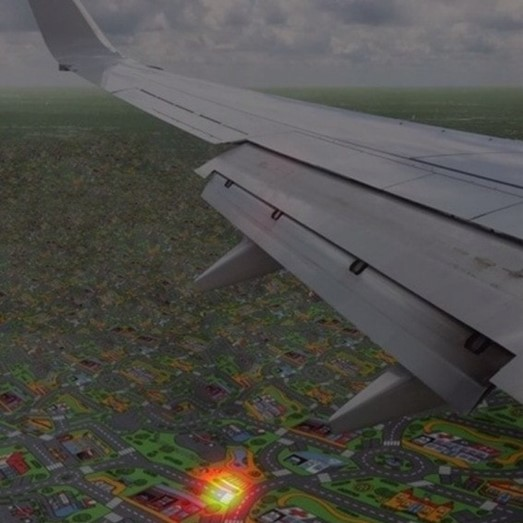
\includegraphics[width=0.8\textwidth]{figures/Bild16.jpg}
        \caption{Proband 16 mit Bild 6 und Heatmap}\label{fig:Bild14a}
    \end{subfigure}
    \begin{subfigure}{0.49\textwidth}
        \centering
        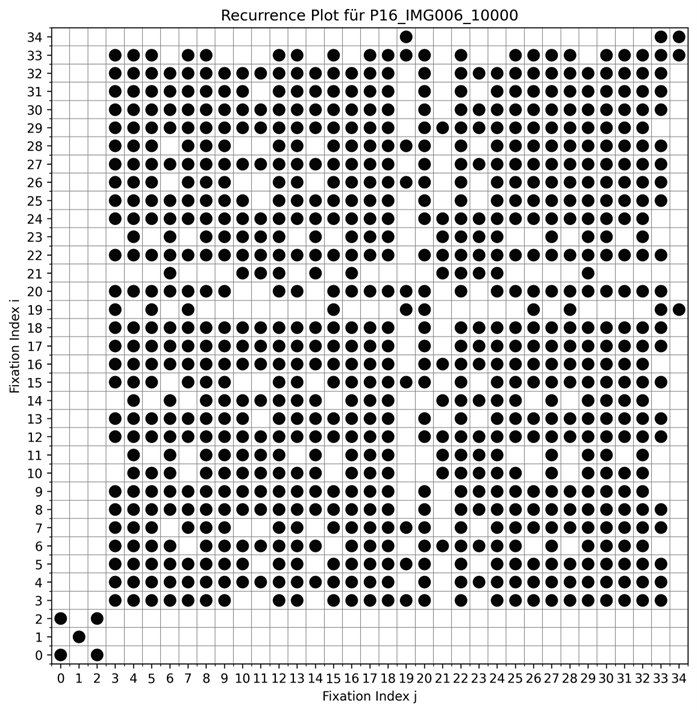
\includegraphics[width=0.8\textwidth]{figures/Bild17.png}
        \caption{Rekurrenz Plot zu Abbildung \ref{fig:Bild14a}}\label{fig:Bild14b}
    \end{subfigure}\label{fig:Bild14}
    \caption{N = 35, R = 381, REC = 64.03\%, DET = 93.96\%, LAM = 91.99\%, CORM = 31.80\%}
\end{figure}

\subsubsection{Vergleich zwischen Bildkategorien}
In Abbildung \ref{fig:bild15} lässt sich erkennen, dass Bilder mit Text eine höhere Anzahl an Fixationen haben, 
dies wird besonders deutlich ab mehr als 50 Fixationen. 
Die recurrence dagegen ist für Bilder mit Text deutlich niedriger (Abb. \ref{fig:bild16}). 
Im Kontext der Bildbetrachtung bedeutet dies, dass sich Texte je länger sie sind, 
seltener mehrmals durchgelesen werden.  Schaut man auf die Korrelationsmatrix in Abbildung \ref{fig:Bild12}, 
bestätigt sich der Trend der sinkenden recurrence mit steigender Fixationsanzahl. 
Der niedrigere corm Wert (Abb. \ref{fig:bild17}) ergibt sich vermutlich daraus, dass Textelemente 
nur einmal komplett am Anfang der Bildbetrachtung gelesen werden. Das reicht, 
um den Wert trotz nachfolgender normaler Betrachtung der Bildelemente zu senken (siehe Abb. \ref{fig:Bild18a} und \ref{fig:Bild18b}). 

\begin{figure}[h]
    \centering
    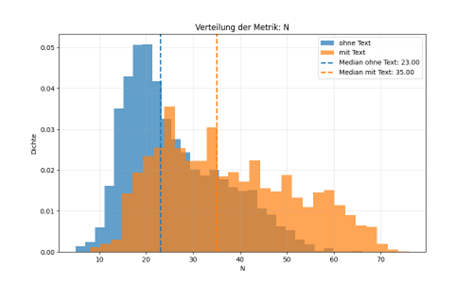
\includegraphics[width=\linewidth,height=0.8\textheight,keepaspectratio]{figures/Bild18.png}
    \caption{Histogramm Vergleich nach Text und Fixationsanzahl N}\label{fig:bild15}
\end{figure}
\begin{figure}[h]
    \centering
    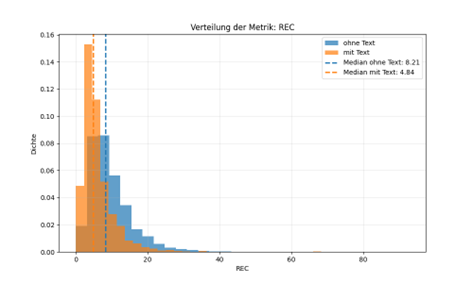
\includegraphics[width=\linewidth,height=0.8\textheight,keepaspectratio]{figures/Bild19.png}
    \caption{Histogramm Vergleich nach Text und recurrence REC}\label{fig:bild16}
\end{figure}
\begin{figure}[h]
    \centering
    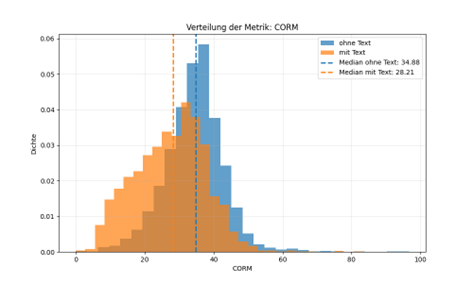
\includegraphics[width=\linewidth,height=0.8\textheight,keepaspectratio]{figures/Bild20.png}
    \caption{Histogramm Vergleich nach Text und corm}\label{fig:bild17}
\end{figure}

\begin{figure}[ht]
    \centering
    \begin{subfigure}{0.49\textwidth}
        \centering
        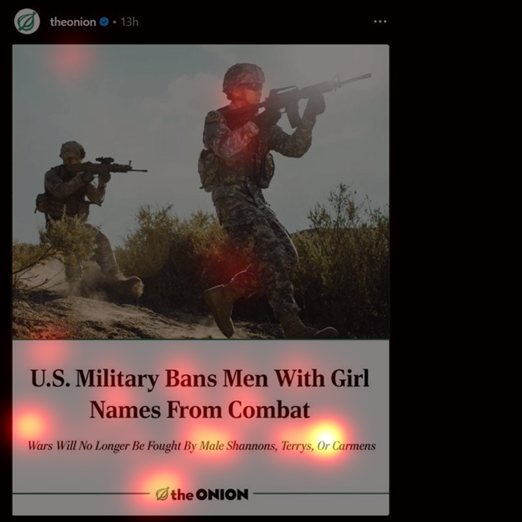
\includegraphics[width=0.8\textwidth]{figures/Bild21.png}
        \caption{Proband 40 mit Bild 124 und Heatmap}\label{fig:Bild18a}
    \end{subfigure}
    \begin{subfigure}{0.49\textwidth}
        \centering
        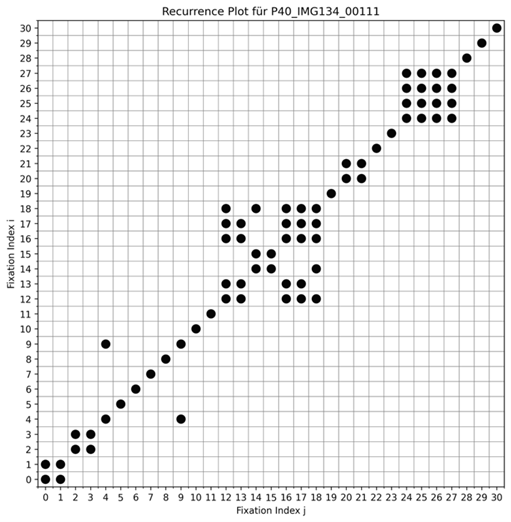
\includegraphics[width=0.8\textwidth]{figures/Bild22.png}
        \caption{Rekurrenz Plot zu Abbildung \ref{fig:Bild18a}}\label{fig:Bild18b}
    \end{subfigure}\label{fig:Bild18}
    \caption{N = 31, R = 21, REC = 4.52\%, DET = 47.62\%, LAM = 54.76\%, CORM = 7.94\%}
\end{figure}

Beim Vergleich von Bildern mit und ohne Person, sticht eine deutlich höhere laminarity heraus (Abb. \ref{fig:bild19}). 
Dies liegt vermutlich daran, dass vor allem Gesichter im Verlauf der Bildbetrachtung erneut genauer betrachtet werden. 

\begin{figure}[h]
    \centering
    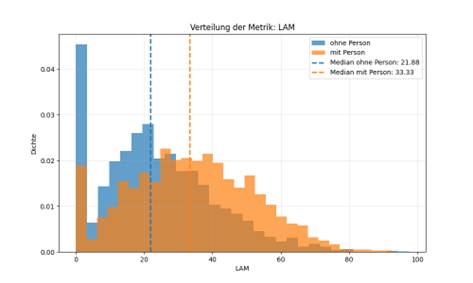
\includegraphics[width=\linewidth,height=0.8\textheight,keepaspectratio]{figures/Bild23.png}
    \caption{Histogramm Vergleich nach Person und laminarity LAM}\label{fig:bild19}
\end{figure}

Beim Vergleich von Bildern nach Ort ist auffällig, dass Bilder mit Ort bei determinism und laminarity 
prozentual mehr als die doppelte Anzahl an „fast Null-Werten“ haben als ohne Ort (Abb. \ref{fig:Bild20a} und \ref{fig:Bild20b}), 
obwohl die recurrence nur um 1,52\% sinkt. Dies könnte daran liegen, dass die AOIs bei reinen 
Orts-/ Landschaftsbildern oft verstreuter und unklarer sind. 

\begin{figure}[ht]
    \centering
    \begin{subfigure}{0.49\textwidth}
        \centering
        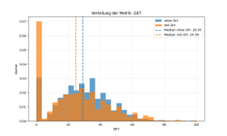
\includegraphics[width=0.8\textwidth]{figures/Bild24.png}
        \caption{Histogramm Vergleich nach Ort und determinism DET }\label{fig:Bild20a}
    \end{subfigure}
    \begin{subfigure}{0.49\textwidth}
        \centering
        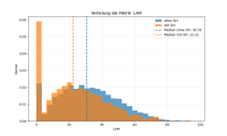
\includegraphics[width=0.8\textwidth]{figures/Bild25.png}
        \caption{Histogramm Vergleich nach Ort und laminarity LAM}\label{fig:Bild20b}
    \end{subfigure}\label{fig:Bild20}
    \caption{Vergleich der Histogramme mit Ort}
\end{figure}

Für Memes lassen sich die Unterschiede darauf zurückführen, dass diese oft Text, während politische Bilder oft Personen enthalten.  

\subsection{Limitationen}
Die RQA-Ergebnisse sind sehr umfangreich und „hoch-aggregiert“, weshalb diese Analyse und 
Interpretation der Ergebnisse nicht alle Auffälligkeiten und Zusammenhänge behandelt. 

\section{Segmentation}

\textbf{Hypothese:} Probanden zeigen eine höhere Anzahl von Fixationen auf den erkannten Personenmasken im Vergleich zu anderen Bildbereichen.

\subsection{Methodik}
Dieses Teil widmet sich der Blickverhaltensanalyse innerhalb der Personen Segmentation mit Hilfe des Segmentation Models 
YOLOv8 verbunden mit den gesammelten Eye-Tracking Daten. Aus den validen 7.443 aufgezeichneten Versuchen haben wir das 
Bincode-Suffix jedes Identifikators entschlüsselt und nur Stimuli beibehalten die Teil der Personenkategorie waren. 
Die Versuche wurden anschließend auf nicht leere Masken überprüft; 48 Bilder mit leeren Vorhersagen wurden verwor-fen, 
sodass 4.593 Versuche aus 104 einzigartigen Stimuli übrig blieben. Diese Filterung stellte sicher, dass nachgelagerte 
Schätzungen echte Personeninhalte abfragten und die Interpretation maskenabhängiger Metriken geschützt wurde.

Für die verbleibenden Versuche haben wir die Blickkoordinaten auf Segmentierungspixel abgebildet, die Anzahl 
und Dauer der Fixierungen innerhalb und außerhalb der Masken gezählt und diese Anteile nach Maskenfläche normalisiert. 
Die durchschnittliche Maskenabdeckung betrug 0,378 der Stimulusebene, was als Null-Erwartung bei gleichmäßiger 
Betrachtung diente. Dennoch richteten die Beobachter 61,2 Prozent ihrer Fixationen auf die Personenbereiche, 
was zu einem mittleren Überschuss von 0,234 über der Flächenbasislinie führte. Zeitbasierte Messungen spiegelten 
dieses Muster wider: Die Teilnehmer verbrachten 65,5 Prozent ihrer Verweildauer auf den Masken, 0,263 mehr als der 
oberflächengewichtete Referenzwert. Selbst das untere Quartil der Teilnehmer verzeichnete Dichteverhältnisse von 
mehr als eins, was die Konsistenz der Aufmerksamkeitsverzer-rung belegt.

\subsection{Ergebnisse}
Abbildung \ref{fig:bild21} fasst die Verteilung der Fixationsüberschüsse zusammen. Das Histogramm liegt überwiegend rechts von Null, 
da 3.943 der 4.593 Versuche einen positiven Überschuss ergeben. Der lange rechte Teil spiegelt Szenen wider, 
in denen kompakte Personensegmente den Blick monopolisierten. Defizite, die in 650 Versuchen auftreten, 
entstehen in der Regel, wenn Masken große Hintergrundbereiche abdecken, die die Bereichsnormalisierung verwässern, 
doch selbst in diesen Fällen wird den Personen immer noch beträchtliche absolute Aufmerksamkeit geschenkt.

\begin{figure}[h]
    \centering
    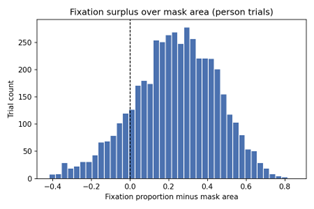
\includegraphics[width=\linewidth,height=0.8\textheight,keepaspectratio]{figures/Bild26.png}
    \caption{Verteilung der Fixationsüberschüsse }\label{fig:bild21}
\end{figure}

Abbildung \ref{fig:bild22} stellt den Fixationsanteil gegenüber der Maskenabdeckung dar. Die meisten Punkte liegen über der Identitätslinie, 
was zeigt, dass die Fixationsanteile über das gesamte Abdeckungsspektrum hinweg die Maskenflächen übersteigen. Masken, 
die weniger als 20 Prozent der Pixel einnahmen, zogen immer noch mehr als 40 Prozent der Fixationen auf sich, während Masken, 
die mehr als die Hälfte des Bildschirms bedeckten, überproportional vertreten blieben. Die Streuung bestätigt somit, 
dass die Segmentierungspipeline semantisch reichhaltige Bereiche isoliert, die den Betrachter unabhängig von ihrer Größe leiten.

\begin{figure}[h]
    \centering
    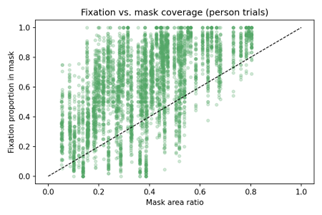
\includegraphics[width=\linewidth,height=0.8\textheight,keepaspectratio]{figures/Bild27.png}
    \caption{Fixationsanteil gegenüber der Maskenabdeckung}\label{fig:bild22}
\end{figure}

Um die Stärke dieser Abweichungen zu formalisieren, haben wir Einstichproben-Z-Tests auf die Fixations- 
und Dauerüberschüsse angewendet. Standardfehler von 0,00318 und 0,00335 ergaben Z-Statistiken von 
73,67 und 78,65, was unter der Normalapproximation zu p-Werten führte, die effektiv gleich Null waren. 
Auf Bildebene erreichten 37 der 94 analysierten Personenbilder durchschnittliche Fixationsüberschüsse von 
mindestens 0,300, während nur neun leicht unter Null fielen, typischerweise wenn Masken diffuse Hintergründe 
umhüllten oder Figuren teilweise verdeckt waren. Diese Ergebnisse bestätigen, dass computergestützt 
erkannte Personen eng mit den Blickprioritäten des Menschen übereinstimmen und bringen eine kleine 
Gruppe von Ausreißern hervor für weitere qualitative Folgeuntersuchungen. Insgesamt zeigt die 
Integration von Segmentierung bei Eye-Tracking, dass Masken den fokalen Inhalt der betrachteten 
Szenen erfassen und dass die Betrachter diesen Bereichen wesentlich mehr Aufmerksamkeit schenken, als die 
Oberflächenabdeckung allein vermuten lässt.

\section{Scanpaths}
 
\textbf{Hypothese:} Scanpaths von Bildern einer Kategorie sind ähnlicher untereinander als Scanpaths von Bildern anderer Kategorien.

--- Variability (Intra-Stimulus Distance) ---
 
Most VARIABLE Stimulus:      'id086'
  - Average distance between its probands: 0.5394
  - Interpretation: Gaze behavior for this stimulus was the most inconsistent across different people.
 
Most CONSTANT Stimulus:      'id144'
  - Average distance between its probands: 0.2823
  - Interpretation: Gaze behavior for this stimulus was the most consistent and predictable across people.
 
 
--- Uniqueness (Inter-Stimulus Distance) ---
 
Most UNIQUE ('Distant') Stimulus: 'id008'
  - Average distance to all other stimuli: 0.5445
  - Interpretation: The gaze behavior for this stimulus was the most distinct from the typical gaze behavior seen across the entire dataset.
 
Most AVERAGE ('Typical') Stimulus: 'id012'
  - Average distance to all other stimuli: 0.4691
  - Interpretation: The gaze behavior for this stimulus was the most representative of the overall average gaze behavior.


\section{Text}

\subsection{Hypothese 1}
Text auf Bildern zieht Aufmerksamkeit auf sich

\subsubsection{Methodik}
Um die Hypothese zu beantworten, muss zuerst bestimmt werden, was überhaupt Text ist. 
Dazu wurde der Text auf jedem Bild händisch markiert. Aus diesen Daten wurden nun für 
jedes Bild zwei werte berechnet, die als Grundlage für viele der Folgenden Analysen dienen: 
Der Textanteil des Bildes und der Prozentteil der Fixationen auf Text. 

\subsubsection{Ergebnisse}
Basierend auf diesen beiden Werten kann nun untersucht werden ob Texte die Aufmerksamkeit 
der Probanden auf sich gezogen haben. Dazu wurden auf Abbildung \ref{fig:bild23} alle untersuchten Bilder geplottet. 
Die X-Achse beschreibt den Textanteil, während die Y-Achse den Fixation-auf-Text Anteil beschreibt. 

\begin{figure}[h]
    \centering
    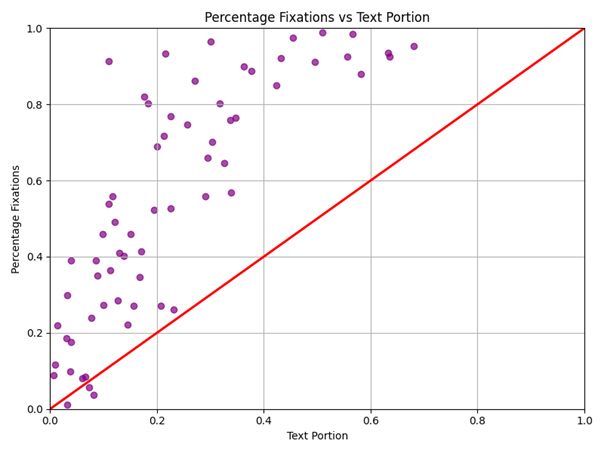
\includegraphics[width=\linewidth,height=0.8\textheight,keepaspectratio]{figures/Bild28.png}
    \caption{Vergleich Text Anteil mit Anteil Fixationen auf Text}\label{fig:bild23}
\end{figure}

Sollte Text keinen Einfluss auf das Blickverhalten haben sollte der Fixation-auf-Text Anteil im Mittel 
etwa gleich dem Textanteil sein. Sollte der Fixationsanteil auf Text allerdings erkennbar höher sein, 
als der Textanteil kann ein Zusammenhang angenommen werden.
Erkennbar ist, dass die Punkte (außer einzelne Ausreißer im Bereich der niedrigen Textanteile) 
alle deutlich links von der Linie liegen. Demnach kann ein Zusammenhang angenommen werden.

\subsection{Hypothese 2}
Verschiedene Arten von Bildern haben Einfluss auf das Blickverhalten

\subsubsection{Methodik}
Dazu wurden die Bilder in verschiedene Gruppen unterteilt:
\begin{itemize}
    \item Nur Text: Text im Vordergrund. Der Hintergrund ist generisch und häufig einfarbig. 
    \item Text Hauptbestandteil: Text im Vordergrund. Der Hintergrund hat nichts mit dem Inhalt zu tun. Häufig handelt es sich um Landschaftsbilder. 
    \item Text/Bild Kombination: Text und Bild hängen zusammen. Da die Bilder der Gruppe große Unterschiede aufweisen wird der Abschnitt weiter unterteilt in Memes und Zitate mit Person (Nur Bilder mit Zitat und zugehöriger Person).
    \item Text Hintergrund: Der Text spielt nur eine Untergeordnete Rolle. 
\end{itemize}

\subsubsection{Ergebnisse}
In Abbildung \ref{fig:bild24} sind die beiden Variablen Text Anteil und Fixation-auf-Text Anteil für jede Gruppe geplottet. 
Die Kategorien unterscheiden sich deutlich.

\begin{figure}[h]
    \centering
    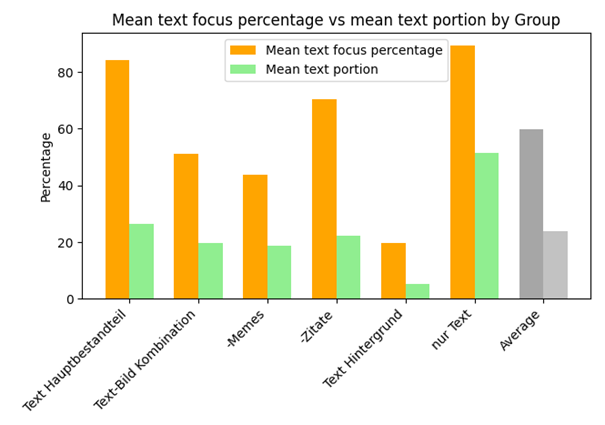
\includegraphics[width=\linewidth,height=0.8\textheight,keepaspectratio]{figures/Bild29.png}
    \caption{Vergleich Fixationen-auf-Text Anteil und Text Anteil}\label{fig:bild24}
\end{figure}

Die nur Text Gruppe hat mit 51,46\% den Höchsten Textanteil, gefolgt von Text Hauptbestandteil 
mit 26,42\%. Trotz dieses Unterschiedes liegt der Fixation-auf-Text Anteil bei der Gruppe 
nur Text mit 89\% nur um etwa 5\% höher als bei Text Hauptbestandteil. Bei beiden Gruppen ist der 
Text das primäre Bildelement und der inhaltslose Hintergrund lenkt offenbar nur wenig ab. 

Um das Verhältnis zwischen den Variablen weiter zu untersuchen ist in Abbildung \ref{fig:bild25} die Rechnung 
(Fixationen-auf-Text Anteil) / (Text Anteil) für die verschiedenen Gruppen aufgeschlüsselt. 
Hier ist vor allem der Wert von Text Hintergrund auffällig. Diese Kategorie hat den niedrigsten 
Text Anteil, allerdings ist der Fixationen-auf-Text Anteil prozentual am höchsten. Das heißt, 
dass überproportional viel Zeit auf dem Wenigen Text dieser Bilder geschaut wird und das, 
obwohl Text in diesen Kategorien lediglich eine Untergeordnete Rolle spielt. Auch auffällig 
ist der vergleichsweise niedrige Wert von Memes. Diese haben einen nur minimal geringeren 
Textanteil als zum Beispiel Zitate, dennoch ist der Fixationen-auf-Text Anteil deutlich niedriger. 
Das spricht dafür, dass das Bild hier wichtiger ist als bei den meisten anderen Kategorien.

\begin{figure}[h]
    \centering
    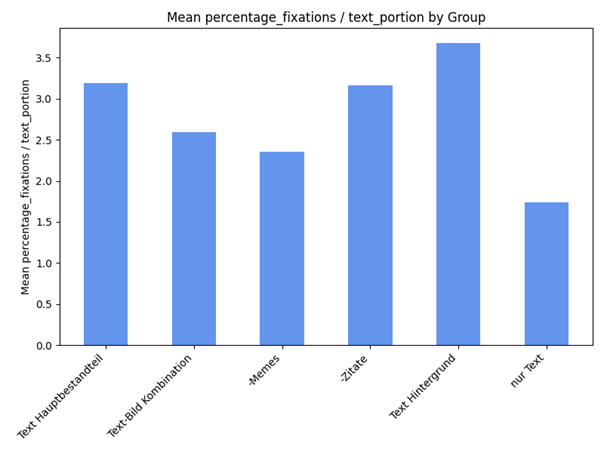
\includegraphics[width=\linewidth,height=0.8\textheight,keepaspectratio]{figures/Bild30.png}
    \caption{Fixationen-auf-Text Anteil/Text Anteil}\label{fig:bild25}
\end{figure}

\subsection{Hypothese 3}
Über den Zeitlichen Verlauf werden Bilder anders betrachtet

\subsubsection{Ergebnisse}
Zuletzt wird das Blickverhalten über den Zeitlichen Verlauf betrachtet. In Abbildung \ref{fig:bild26} kann der 
Anteil der Fixationen-auf-Text für jeden Zeitpunkt betrachtet werden. Das heißt, dass zum Beispiel 
für Memes 40\% aller Gaze Points an der Stelle 200 auf Text lagen. 

\begin{figure}[h]
    \centering
    
\includegraphics[width=\linewidth,height=0.8\textheight,keepaspectratio]{figures/Dummy.jpg}
    \caption{Fixationen-auf-Text Anteil/Text Anteil}\label{fig:bild26}
\end{figure}

Im Zeitlichen Verlauf ist ein starker Trend zu erkennen. Anfangs steigt der gaze-point-auf-Text Anteil stark an und erreicht 
bereits in den ersten Sekunden seinen Hochpunkt. Anschließend sinkt der Anteil wieder relativ schnell. 
Diese Ausprägung ist in verschiedenen Stärken zu beobachten. Besonders auffällig ist hierbei die Kategorie Memes. 
Bereits bei Gaze-point 50 erreicht diese den Hochpunkt von etwa 70\%. Im Verlauf der nächsten Sekunden 
mehr als halbiert sich dieser Anteil auf nur noch etwa 30\%. Das liegt vermutlich daran, dass zuerst der Text 
gelesen und anschließend das dazugehörige Bild betrachtet wird. Bei Zitaten dauert der Hochpunkt länger an, 
bevor auch hier der Anteil wieder stark abfällt. Die verlängerte Hochphase kann mit der größeren Menge an Text 
und zusammenhängenden Sätzen erklärt werden. Einzig die nur Text Kategorie verzeichnet kaum Schwankungen, 
was Sinn ergibt, da es außer Text keinen Inhalt gibt, der Betrachtet werden kann. 

\section{Fazit}

Die durchgeführten Analysen haben gezeigt, dass Eye-Tracking ein vielfältiges und leistungsfähiges Werkzeug ist, 
um Blickverhalten systematisch zu erfassen und Hypothesen über die Wahrnehmung und Verarbeitung visueller Inhalte 
zu überprüfen. Unser zweistufiges Vorgehen – zunächst explorativ, dann hypothesengeleitet – erwies sich dabei als 
gewinnbringend: Während die explorative Phase Strukturen, Auffälligkeiten und erste Muster sichtbar machte, 
konnten in der hypothesenorientierten Phase diese Beobachtungen gezielt überprüft und quantifiziert werden. 

Zentrale Befunde lassen sich wie folgt zusammenfassen: 
\begin{itemize}
    \item Die Betrachtungsdauer nimmt im Verlauf der Bildpräsentation signifikant ab, 
    was auf Ermüdungseffekte oder eine zunehmende Sättigung bei den Teilnehmenden hindeutet. 
    \item Bildkategorien – insbesondere das Vorhandensein von Text oder Personen – 
    beeinflussen das Blickverhalten maßgeblich. Text zieht die Aufmerksamkeit in besonderem Maße auf sich, 
    wobei die Wirkung je nach Kontext (Hintergrundtext, Meme, Zitat) variiert. 
    \item Kontrastmerkmale wie RMS und Laplace korrelieren signifikant mit Fixationsmustern 
    und deuten auf ein exploratives Scanning-Verhalten bei detailreichen Bildern hin. 
    \item Rekurrenzanalysen zeigen, dass Bildinhalte wie Text und Gesichter zu charakteristischen 
    Mustern wiederholter Fixationen führen, während landschaftliche Szenen eher durch eine zerstreute 
    Betrachtung gekennzeichnet sind. 
    \item Segmentierungsbasierte Analysen bestätigen, dass Personen in Bildern 
    den Blick der Teilnehmenden besonders stark binden – unabhängig von der relativen Flächenabdeckung. 
\end{itemize}

Insgesamt verdeutlichen die Ergebnisse, dass Blickverhalten kein zufälliger Prozess ist, 
sondern systematisch durch Bildmerkmale, Präsentationsbedingungen und Kategorien geprägt wird. 
Die Kombination aus klassischen Kennwerten, statistischen Modellierungen und innovativen Verfahren 
wie der Rekurrenzanalyse oder der Segmentierung eröffnet dabei neue Perspektiven für die 
Aufmerksamkeitsforschung. 

Für zukünftige Arbeiten erscheint es vielversprechend, die Ansätze durch größere Datensätze, 
eine stärkere Berücksichtigung individueller Unterschiede sowie multimodale Methoden (z.\,B. EEG, 
Verhaltensmaße) zu erweitern. So ließe sich noch präziser untersuchen, wie Menschen visuelle 
Informationen wahrnehmen, verarbeiten und bewerten.  

Unsere Studie zeigt: Eye-Tracking ermöglicht nicht nur die Erfassung von Blickbewegungen, 
sondern liefert tiefe Einblicke in kognitive Prozesse der Aufmerksamkeit und Wahrnehmung – 
und trägt damit zu einem besseren Verständnis menschlicher Informationsverarbeitung bei. 


\newpage
\printbibliography[heading=header]

% ============================================================

\end{document}